\documentclass[11pt]{article}
\usepackage{fullpage,graphicx,psfrag,amsmath,amsfonts,verbatim}
\usepackage[small,bf]{caption}
\usepackage[compact]{titlesec}

\input defs.tex

\bibliographystyle{ieeetr}

\title{Bitcoin UTXO Lifespan Prediction}
\author{Robert Konrad \& Stephen Pinto}

\begin{document}
\maketitle

\section{Background \& Motivation}
The Bitcoin crypto currency~\cite{Na:08,NBF:15} is the most widely used and highly valued digital currency in existence. Every day sees thousands of transactions added to the blockchain. The blockchain is a global, agreed-upon ledger of every transaction that has ever occured and is continually extended as a single linked list. Each transaction in the blockchain, say Alice paying Bob 10 BTC, has one or more transaction outputs (TXO) which serve as sums of spendable BTC. These unspent sums are called \emph{Unspent Transaction Outputs} (UTXO). They remain UTXOs until the owner (Bob in our example) redeems them to pay someone else (at which time they are referred to as spent TXOs).

\begin{figure}
\begin{center}
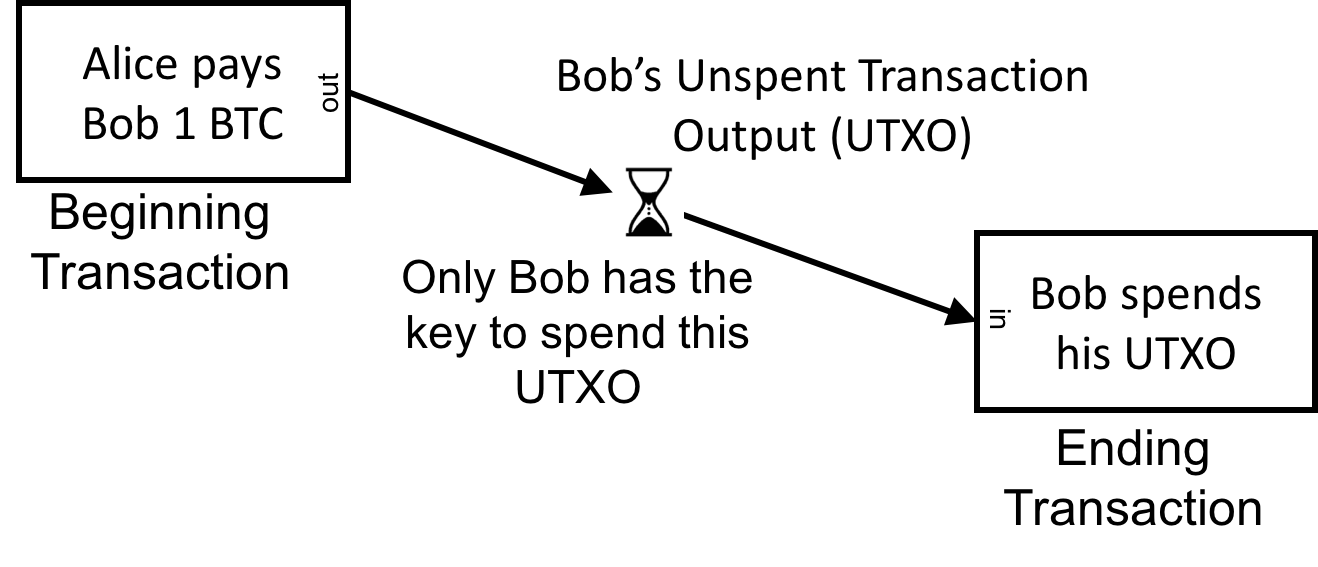
\includegraphics[width=0.5\textwidth]{figures/utxo}
\end{center}
\caption{Illustrated Explanation of a UTXO. An arbitrary amount of time may pass before Bob spends his UTXO.}
\label{utxo}
\end{figure}

This project seeks to predict how long a TXO will remain unspent. More formally, given some information about the beginning transaction which created the UTXO and some information about the Bitcoin market on the day of its creation, this project predicts which of ten broad time scales the UTXO lifespan will fall into. This predictor could inform broader applications such as anomaly/fraud detection, trade volume and volatility prediction, and the modelling of individual spending habit. The Bitcoin industry is worth billions of dollars and growing rapidly. Possible insights into the previosly mentioned topics would be of use to any number of financial institutions involved in the future of cryptocurrencies. 



\section{Dataset \& Features}
One of the (many) blockchain explorers, Blockchain.info, has a public API exposing data about individual transactions as well as general Bitcoin market statistics. A python script queried Blockchain.info at a polite rate to gather 13146 training samples and then exported the data to a Matlab readable format. A Matlab script then curated the data into a matrix with the features listed in figure~\ref{features}. The feature set consists of information pertaining to the individual beginning transactions, and information about the bitcoin market statistics on the day of creation.



\begin{figure}
\begin{center}
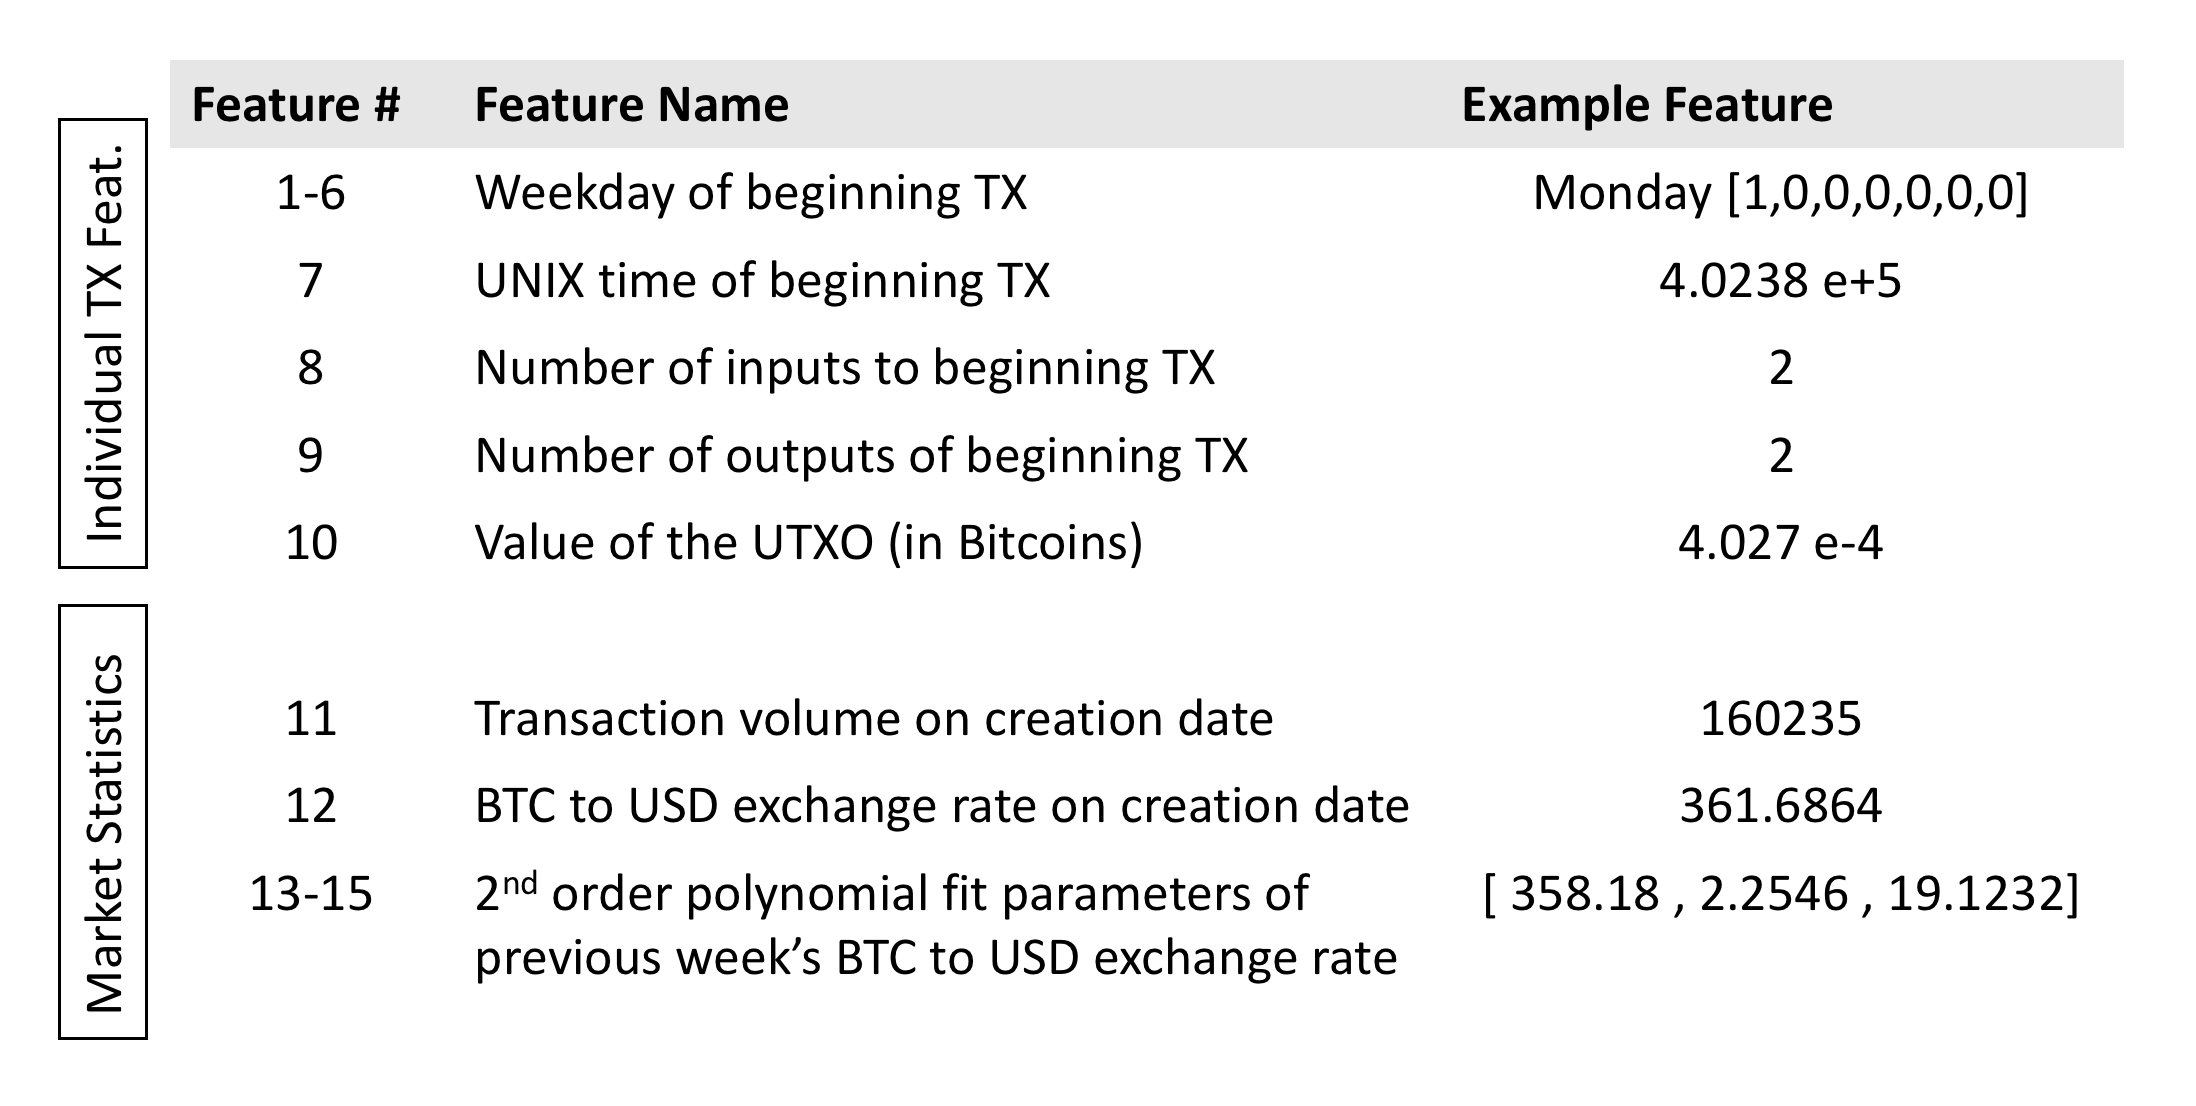
\includegraphics[width=0.7\textwidth]{figures/features}
\end{center}
\caption{The features used as inputs to the classifier .}
\label{features}
\end{figure}



We dummy coded the weekday with the reference day being Sunday. This created 6 new binary features, where each feature dictates whether the transaction occurred on a particular day. Sunday, the reference day, is represented by these 6 features being 0. The UNIX time of beginning transaction corresponded to the number of hours that occurred since the Epoch time, Thursday, 1 January, 1970. The 11th feature, transaction volume on creation date, corresponds to to the total number of unique Bitcoin transactions that occurred on the day of creation. The final three features are the three 2nd order polynomial parameters that fit the last week's USD to BTC conversion rate.


\begin{figure}
\begin{center}
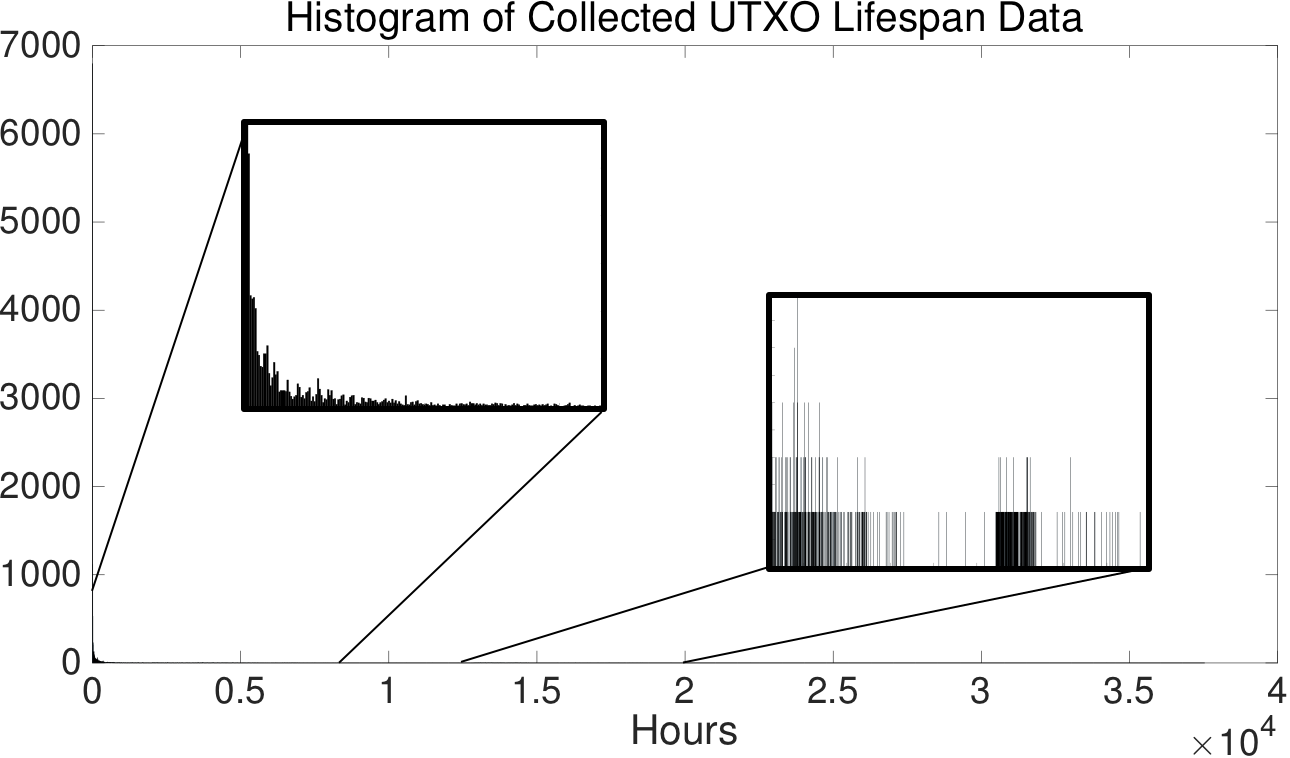
\includegraphics[width=0.6\textwidth]{figures/hist.png}
\end{center}
\caption{The histogram of collected UTXO lifespans with two regions magnified.}
\label{hist}
\end{figure}


\section{Methods}
As shown in figure~\ref{hist}, the tail of the UTXO Lifespan distribution is extremely long. As such, regression might lead to prediction errors that are large enough to remove their useful meaning. Classification into a finite set of lifespan bins (defined by ranges of time) clarifies this issue and provides more intuitive results. The trick, however, is to define useful, data-dependent time ranges. Hardcoding these based on eyeballing the distribution seemed meaningless so we chose to instead split the full domain into ten equal-probability ranges.

Two methods of doing this are either (1) entirely empirically or (2) based on a fitted distribution. The former case is simply a matter of sorting the lifespan dataset and splitting it into ten equally sized groups. The latter requires more processing. Understanding that the data should show signs of a Laplace or exponential distribution based the standard application of those distributions, the first step was to cluster the lifespan set using k-median ($\ell_1$ penalty function) clustering. From there, we fitted either a Normal, Laplace, or Exponential (whichever was most likely) distribution to each cluster using maximum likelihood estimation and then formed a global distribution as a weighted sum. 

\begin{figure}
\begin{center}
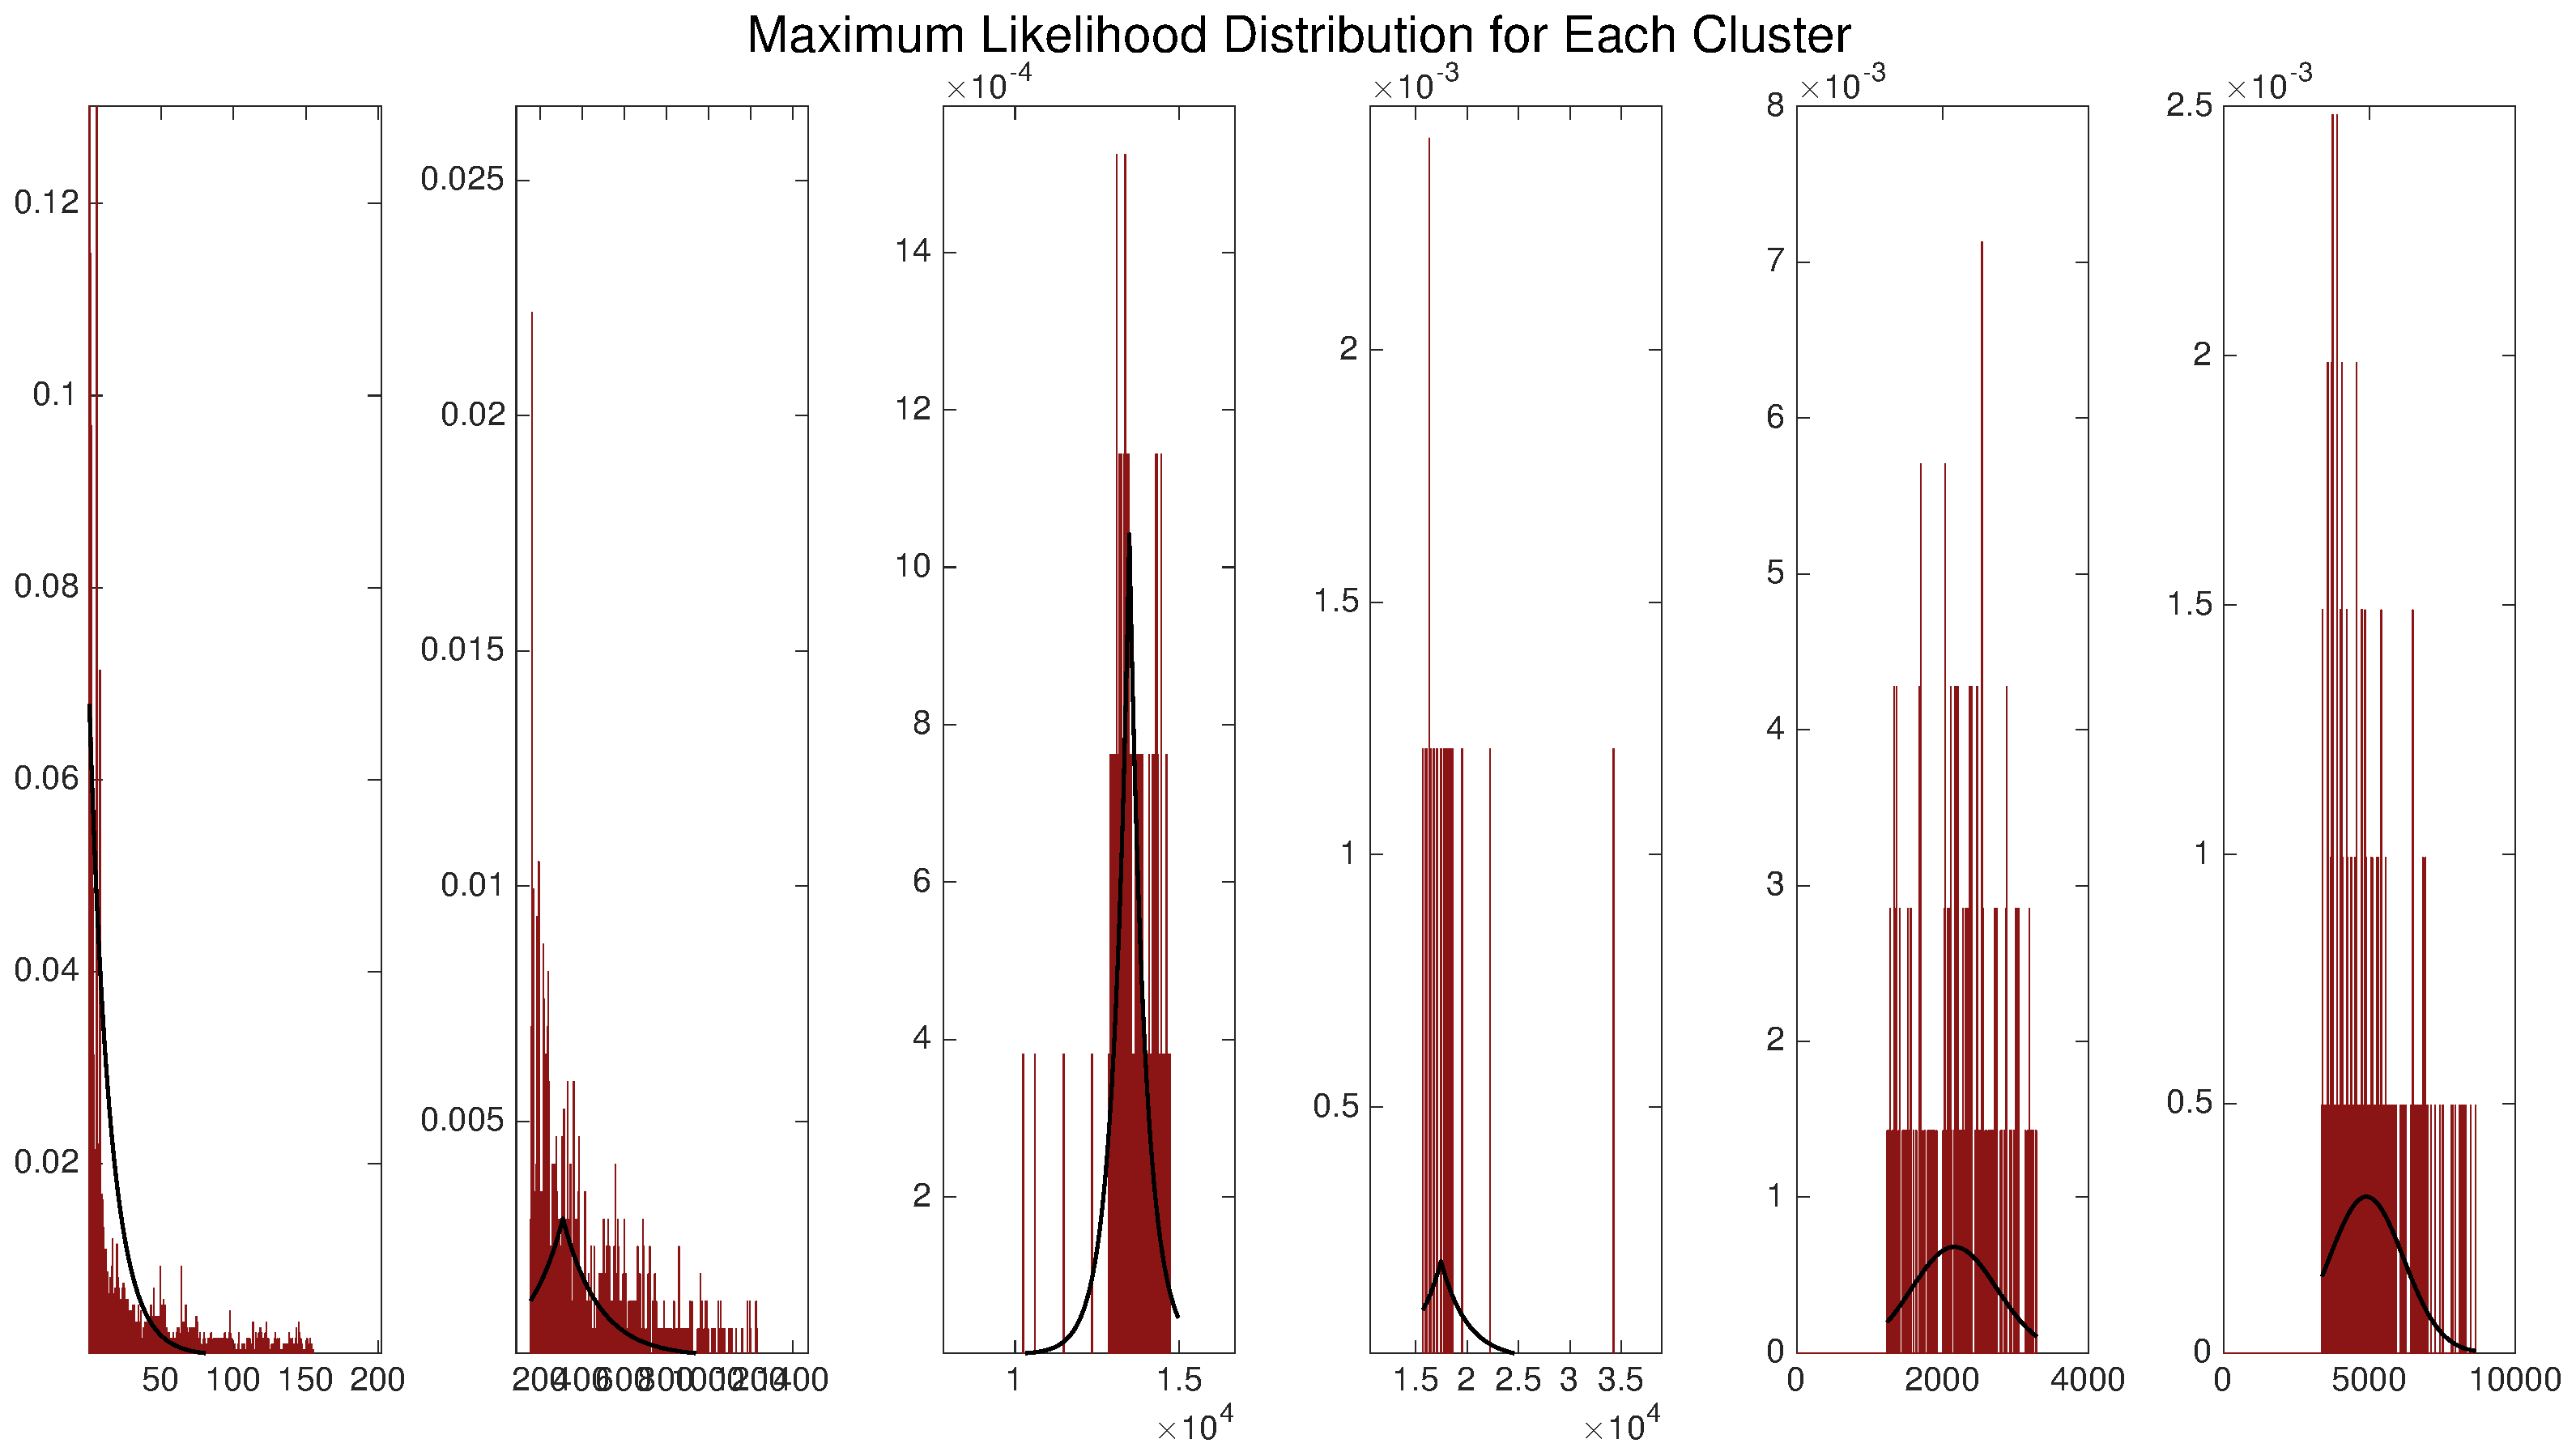
\includegraphics[width=0.8\textwidth]{figures/fits}
\end{center}
\caption{The maximum likelihood distribution fits for each of the six $\ell_1$ penalty clusters.}
\label{fits}
\end{figure}

\begin{table}[!htbp]
\begin{tabular}{|r||c|c|c|c|c|c|c|c|c|c|}
\hline
Upper Bound of Subdomain & 2 m & 10 m & 31 m & 80 m & 3 h & 7 h & 1 d & 3 d & 2 wk & $\infty$\\
\hline
\% of Dataset in Subdomain & 10 & 10 & 10 & 10 & 10 & 10 & 10 & 10 & 10 & 10\\
\hline
\end{tabular}
\caption{Table of subdomain boundaries and the distribution of datapoints within subdomains for empirically calculated subdomains.}
\label{opt1}
\end{table}

\begin{table}[!htbp]
\begin{tabular}{|r||c|c|c|c|c|c|c|c|c|c|}
\hline
Upper Bound of Subdomain & 2 h & 4 h & 6.5 h & 9.5 h & 12.5 h & 17.5 h & 1 d & 1.5 d & 2 wk & $\infty$\\
\hline
\% of Dataset in Subdomain & 44 & 8 & 7 & 5 & 2 & 2 & 3 & 3 & 16 & 10\\
\hline
\end{tabular}
\caption{Table of subdomain boundaries and the distribution of datapoints within subdomains for subdomains from a fitted distribution.}
\label{opt2}
\end{table}

Tables~\ref{opt1} and~\ref{opt2} describe the ten subdomains with raw data and the fitted distribution respectively. Table~\ref{opt2} reveals that the fitted distribution does not sufficiently capture the heavy weighting towards 0 since 44\% of the data is falling into what we hoped was a 10\% probability domain. Keeping in mind that the goal of this subdomain split is to find a meaningful set of lables, the choice between the two options is up to which domains seem more meaningful to a future user. We created two classifiers -- one for each label set.


We used two different classification algorithms: SVM with a (Gaussian) radial basis kernel and softmax regression. The SVM optimization problem is as follows~\cite{Ng:15,HCL:10,BoV:04}:
\begin{align*}
\min_{\gamma,w,b} & \frac{1}{2}||w||^2 + C \sum_{i=1}^{m}\xi_i \\
s.t. & y^{(i)}(w^Tx^{(i)} + b) \ge 1 - \xi_i, \quad i = 1,...,m \\
& \xi_i \ge 0, \quad i = 1,...,m
\end{align*}
With the kernel function $K(x,z) = \exp \left(-\frac{\|x-z\|^2}{2\sigma^2}\right)$. This kernel function implicitly moves the feature set to a high dimensional space where the optimal margin between classes is larger and better fit by a linear equation than in the original, low dimentional space. 

Softmax regression is a GLM that can be run on a multinomial dataset. In class we saw that if we dummy coded our labels (with one being a reference label), then we could express the multinomial distribution as a member of the exponential family. The softmax function, $\phi_i = \frac{e^{\eta_i}}{\sum_{j=1}^{k}e^{\eta_j}}$, where $\eta$ is the natural parameter and $k$ is the number of labels, is found to describe the conditional distribution of $y$ given $x$ : 
\begin{align*}
     p(y=i | x; \theta) &= \frac{e^{\eta_i}}{\sum_{j=1}^{k}e^{\eta_j}} =
     \frac{e^{\theta_i^Tx}}{\sum_{j=1}^{k}e^{\theta_j^Tx}}
\end{align*}
With this conditional probablity we are able to estimate the probablity of a certain feature set falling into each category, $i$.


\section{Results}
\begin{figure}
\begin{center}
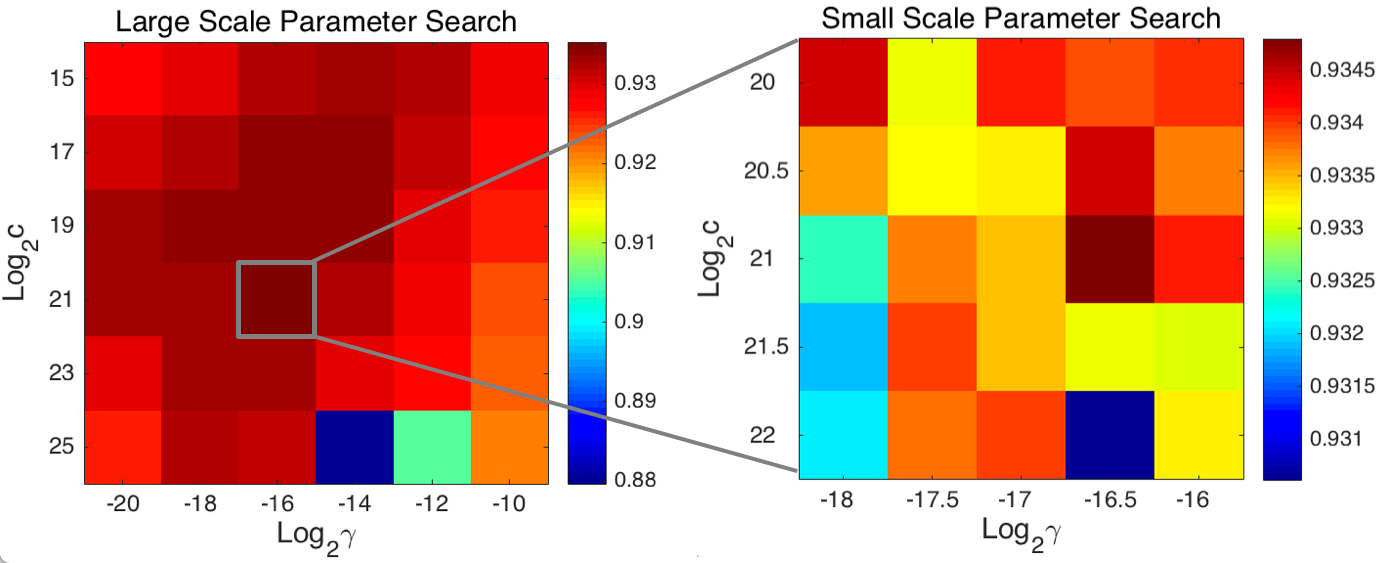
\includegraphics[width=0.7\textwidth]{figures/paramSearch}
\end{center}
\caption{Classifier performance vs $\gamma$ and $C$. One region of the broader heatmap is magnified for higher granularity.}
\label{paramSearch}
\end{figure}

SVM with a radial kernel performed significantly better than any other tested alternative so this section highlights only those results on the empirically decided equal-probability labels. The parameters $\gamma$ and $C$ changed the predication accuracy as they varied so figure~\ref{paramSearch} highlights the process of first training and 5-fold validating on a rough range of the two, then zooming in for finer changes to find an ideal pair of values at $\gamma = 1.9 \times 10^{-6}$ and $C = 4.2 \times 10^{6}$. 

\begin{figure}
\begin{center}
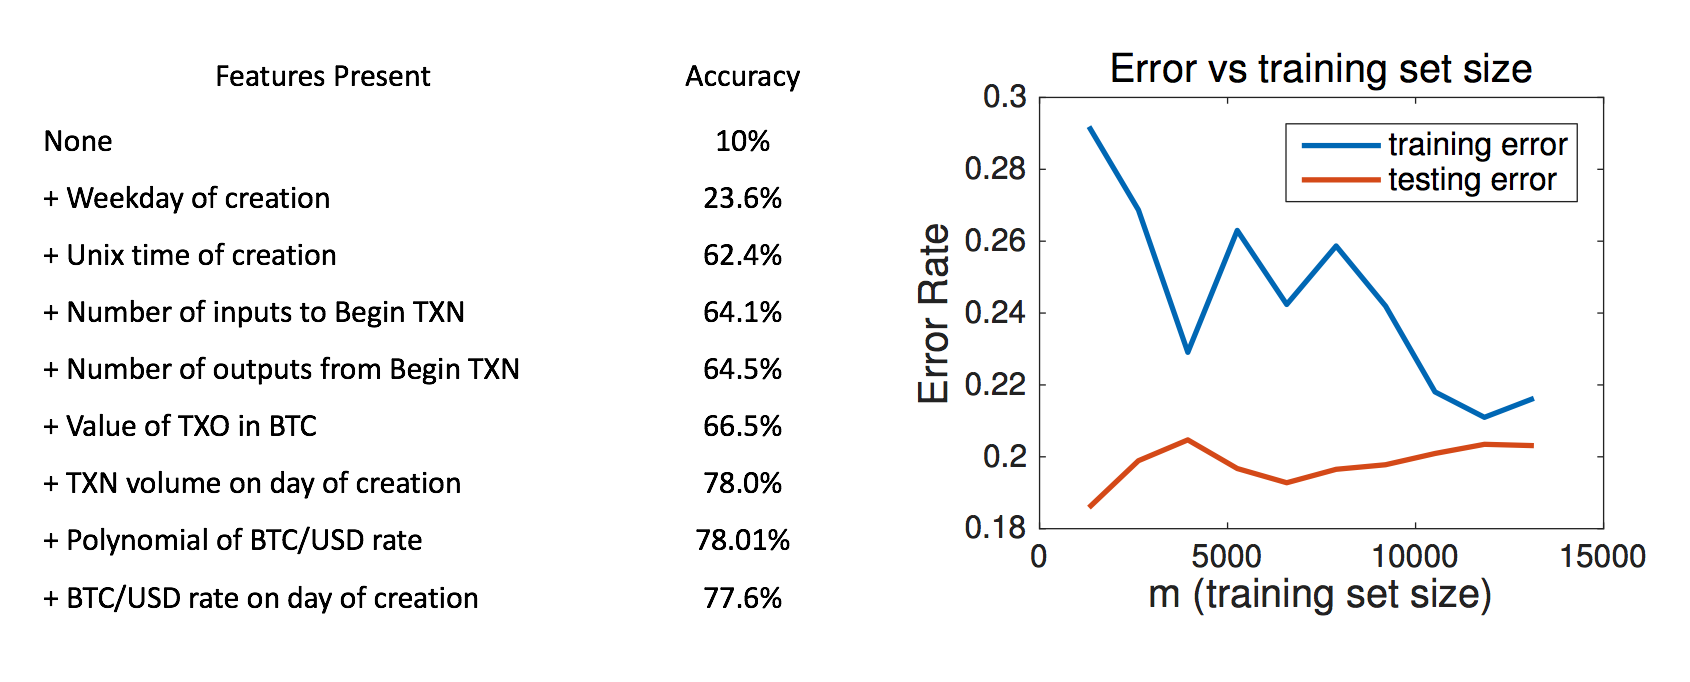
\includegraphics[width=0.9\textwidth]{figures/accuracy}
\end{center}
\caption{The accuracy of the SVM classifier using empirical labels with the sequential addition of features and the training/test error vs dataset size.}
\label{accuracy}
\end{figure}

Figure~\ref{accuracy} shows the training and test error with respect to training set size with the peak $\gamma$ and $C$ pair as well as the effect of each feature on prediction accuracy as the features are added in one by one. Since space is scarce, suffice to say we have corresponding plots of figures~\ref{paramSearch} and~\ref{accuracy} for the fitted-distribution-defined equal probability labels. The baseline accuracy (\ie predicting label 1 every time) is 44\% while the peak accuracy with all features present is about 95\%. Using other classifiers -- softmax regression, linear SVM kernel, 3rd degree polynomial SVM kernel, and sigmoid SVM kernel -- we had prediction accuracies 43\%, 35\%, 34\%, and 9\% respectively. 

\section{Conclusion \& Future Work}
It would be interesting to study the stationarity (or lack-there-of) of the UTXO Lifespan distribution (\ie are typical spending habits varying over Bitcoin history?) Such information might help with finding a better fitting underlying distribution that would be more robust than relying on equal-probability binning of raw data. Similarly, attempting to model the underlying distribution as a mixture of Laplace distributions might make more sense than fitting a set of adjacent clusters with individual distributions. We started down that path and would like to acknowledge Junjie Qin's help but we were unable to bring it to a useful state. It would also be worth see how many equal-probability bins we can meaningfully classify into (the more the better). Finally, two interesting follow up projects would be to use this prediction tool to create expected volatility plots of the Bitcoin market or pairing this predictor with de-anonymizing tools to form individual spending models for clustered entities on the blockchain.

\newpage

\bibliography{btc-learning}

\end{document}